%%%%%%%%%%%%%%%%%%%%%%%%%%%%%%%%%%%%%%%%%%%%%%%%
% E.Pinault-Bigeard - e.pinault-bigeard@upsti.fr
% http://s2i.pinault-bigeard.com
% CC BY-NC-SA 2.0 FR - http://creativecommons.org/licenses/by-nc-sa/2.0/fr/
%%%%%%%%%%%%%%%%%%%%%%%%%%%%%%%%%%%%%%%%%%%%%%%%
\documentclass[11pt, multicol]{article}
%%%%%%%%%%%%%%%%%%%%%%%%%%%%%%%%%%%%%%%%%%%%%%%%
% Package UPSTI_Document
%%%%%%%%%%%%%%%%%%%%%%%%%%%%%%%%%%%%%%%%%%%%%%%%
%%%%%%%%%%%%%%%%%%%%%%%%%%%%%%%%%%%%%%%%%%%%%%%%
% Package UPSTI_Document
%%%%%%%%%%%%%%%%%%%%%%%%%%%%%%%%%%%%%%%%%%%%%%%%
\usepackage{subcaption}
\usepackage[usenames, svgnames, dvipsnames]{xcolor}
\usepackage{UPSTI_Document}
\usepackage{pgfplots}
\usepackage{import}
\definecolor{darkspringgreen}{rgb}{0.09, 0.45, 0.27}

\newcommandx*{\dessinRepereFigGeo}[5][1=\vx{},2=\vy{},3=\vz{},4=,5=0]
	{
		\draw [->,very thick] (0,0) -- (1,0) ;
		\draw [->,very thick] (0,0) -- (0,1) ;
    \fill[white] (0,0) circle (0.13);
    \draw [->,very thick] (0,0) circle (0.13);
    \ifnumequal{#5}{0} {% z vers nous
      \fill[black] (0,0) circle (0.03);
      \draw [->,thick] (0,0) circle (0.04);
    }{% z vers la feuille
  		\begin{scope} [rotate=45]
  			\draw [-,thick] (0,-0.12) -- (0,0.12) ;
  			\draw [-,thick] (-0.12,0) -- (0.12,0) ;
  		\end{scope}
    }
		\draw [anchor=north west] (1.1,0) node {${#1}$};
		\draw [anchor=south west] (0,1.1) node {${#2}$};
		\draw [anchor=north east] (-0.1,0) node {${#3}$};
		\draw [anchor=north west] (-0.1,-0.1) node {${#4}$};
	}

	\usepackage{array}
	\newcolumntype{L}[1]{>{\raggedright\let\newline\\\arraybackslash\hspace{0pt}}m{#1}}
	\newcolumntype{C}[1]{>{\centering\let\newline\\\arraybackslash\hspace{0pt}}m{#1}}
	\newcolumntype{R}[1]{>{\raggedleft\let\newline\\\arraybackslash\hspace{0pt}}m{#1}}

	\usepackage{pifont}% http://ctan.org/pkg/pifont
\newcommand{\cmark}{\color{green}\ding{51}}%
\newcommand{\xmark}{\color{red}\ding{55}}%
\newcommand{\fmark}{\ding{229}}%
\newcommand{\itemc}{\item[\cmark]}%
\newcommand{\itemx}{\item[\xmark]}%
\newcommand{\itemf}{\item[\fmark]}%


%---------------------------------%
% Paramètres du package
%---------------------------------%

% Version du document (pour la compilation)
% 1: Document prof
% 2: Document élève
% 3: Document à publier
\newcommand{\UPSTIidVersionDocument}{2}


% Classe
% 1: PTSI				6: PSI*			11: TSI2		16: Spé
% 2: PT	(par défaut)	7: MPSI			12: ATS
% 3: PT*				8: MP			13: PC
% 4: PCSI				9: MP*			14: PC*
% 5: PSI				10: TSI1		15: Sup
%\newcommand{\UPSTIidClasse}{2}



% Matière
% 1: S2I (par défaut)    2: IPT     3: TIPE
% 6: Vie au lycée
\newcommand{\UPSTIvariante}{5}
\newcommand{\UPSTIidMatiere}{0}
\newcommand{\UPSTIintituleMatiere}{Automatique}
\newcommand{\UPSTIsigleMatiere}{Autom}
% Type de document
% 0: Custom*				7: Fiche Métho de			14: Document Réponses
% 1: Cours (par défaut)		8: Fiche Synthèse    		15: Programme de colle
% 2: TD     				9: Formulaire
% 3: TP						10: Memo
% 4: Colle					11: Dossier Technique
% 5: DS						12: Dossier Ressource
% 6: DM						13: Concours Blanc
% * Si on met la valeur 0, il faut décommenter la ligne suivante:
%\newcommand{\UPSTItypeDocument}{Custom}
\newcommand{\UPSTIidTypeDocument}{1}

% Titre dans l'en-tête


% Titre dans l'en-tête

\newcommand{\UPSTIvariante}{5}

\newcommand{\UPSTItitreEnTete}{Automatisme industriel}
%\newcommand{\UPSTItitreEnTetePages}{}
\newcommand{\UPSTIsousTitreEnTete}{Introduction aux API}


% Titre
%\newcommand{\UPSTItitrePreambule}{Automatisme industriel}
\newcommand{\UPSTItitre}{La programmation d'un Automate Industriel}

% Durée de l'activité (pour DS, DM et TP)
\newcommand{\UPSTIduree}{3h30}

% Note de bas de première page
%\newcommand{\UPSTInoteBasDePremierePage}{Geoffrey Vaquette}
% Numéro (ajoute " n°1" après DS ou DM)
\newcommand{\UPSTInumero}{2}

% Numéro chapitre
%\newcommand{\UPSTInumeroChapitre}{1}

% En-tête customisé
%\newcommand{\UPSTIenTetePrincipalCustom}{UPSTIenTetePrincipalCustom}

% Message sous le titre
%\newcommand{\UPSTImessage}{Message sous le titre}


% Référence au programme
%\newcommand{\UPSTIprogramme}{\EPBComp \EPBCompP{B1-02}, \EPBCompP{B2-49}, \EPBCompS{B2-50}, \EPBCompS{B2-51}, \EPBCompP{C1-07}, \EPBCompP{C1-08}}

% Si l'auteur n'est pas l'auteur par défaut
%\renewcommand{\UPSTIauteur}{WWOOOOOOWW}

% Si le document est réalisé au nom de l'équipe
%\newcommand{\UPSTIdocumentCollegial}{1}

% Source
\newcommand{\UPSTIsource}{G. Vaquette, A. Juton, J. Deprez, J. Maillefert}

% Version du document
\newcommand{\UPSTInumeroVersion}{1.1}

%-----------------------------------------------
\UPSTIcompileVars		% "Compile" les variables
%%%%%%%%%%%%%%%%%%%%%%%%%%%%%%%%%%%%%%%%%%%%%%%%


%%%%%%%%%%%%%%%%%%%%%%%%%%%%%%%%%%%%%%%%%%%%%%%%
% Début du document
%%%%%%%%%%%%%%%%%%%%%%%%%%%%%%%%%%%%%%%%%%%%%%%%
\begin{document}
\UPSTIbuildPage

%\UPSTIobjectif{Durant cette activité, nous allons analyser une trame pour l'envoi d'informations sur une étiquette.}

%\tableofcontents
\section{Pupitre simple (support des premiers TPs)}

\begin{figure}[h!b]
\centering
\includegraphics[width=.4\textwidth]{images/schemaPupitre}
	\caption{Schéma pupitre}
	\label{fig:pupitre}
\end{figure}
Dans le premier TP, vous allez mettre en oeuvre un pupitre opérateur relié à un automate, représenté sur la Figure~\ref{fig:pupitre}

Ce support est composé de :
\begin{itemize}
	\item Un capteur inductif
	\item Trois voyants ($V_0, V_1, V_2$)
	\item Trois boutons poussoirs ($BP_0, BP_1, BP_2$)
	\item Un potentiometre
	\item Un cadrant affichant la tension mesurée par un voltmètre
\end{itemize}

\UPSTIquestion{Faire la liste des organes connectés aux entrées et sorties de l'automates.}
\UPSTIcorrection{\begin{description}
	\item [Entrées : ] Les capteurs
	\begin{itemize}
			\item Un capteur inductif (logique)
			\item Trois boutons poussoirs ($BP_0, BP_1, BP_2$) (logique)
			\item Un potentiometre (analogique)
	\end{itemize}
	\item [Sorties :] Les actionneurs et pré-actionneurs
	\begin{itemize}
		\item Voyants (logique)
		\item Cadrant (analogique)
	\end{itemize}
\end{description}}
\UPSTIquestion{Pour chaque entrée et sortie, indiquer son type (TOR, analogique ou numérique). }
\UPSTIcorrection{Voir question précédente}

\UPSTIquestion{S'agit-il d'une structure locale ou déportée ? Justifier}
\UPSTIcorrection{l s’agit d’une structure locale car les modules d’entrées et de sorties sont directement branchés sur l’automate. Il n’y a pas de bus de terrain entre les modules et l’automate. }

On relit le potentiometre à un convertisseur analogique-numérique (CAN) 8 bits. La tension en sortie du potentiomètre varie entre 0V et 10V.
\UPSTIquestion{Quelle est la valeur maximale en sortie du CAN ?}

\UPSTIcorrection{Il s’agit d’un CAN 8bits, sa valeur maximale en binaire est 0x1111 1111 = 255}

\UPSTIquestion{Si la tension en sortie du potentiomètre est de 5V, quelle est la valeur en sortie du CAN ?}
\UPSTIcorrection{Par un calcul de proportionnalité (rêgle de trois), on trouve $\frac{5.0\times 255}{10}=127.5$ arrondi à $128$}
\UPSTIquestion{Même question pour 3.2V ? }
\UPSTIcorrection{Par un calcul de proportionnalité (rêgle de trois), on trouve $\frac{3.2\times 255}{10}=81.6$ arrondi à $82$}
\UPSTIquestion{Quelle est la fonction de chacun des modules de l'automate ?}
\begin{description}
	\item [CPS2000 : ] Fournir l'énergie électrique à l'automate
	\item [CPU : ] C'est l'organe de commande, l'unité de calcul qui exécute le Programme
	\item [NOC0401 : ] Relier l’automate au réseau Ethernet
\end{description}
\pagebreak
\section{Ascenseur}
\resetNumQuestion
\begin{figure}[h!t]
	\centering
	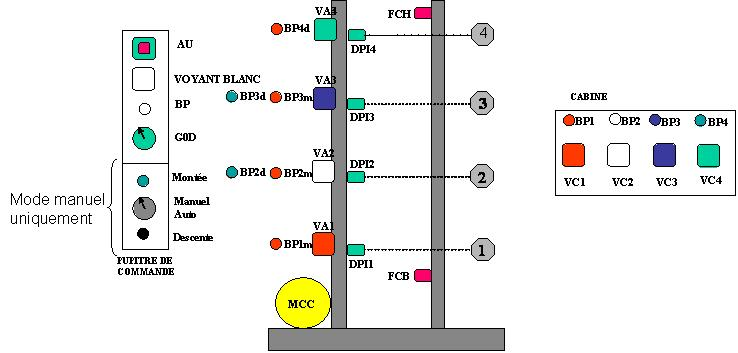
\includegraphics[width=.5\linewidth]{images/ascenseur}
	\caption{Tableau de commande d'un ascenseur}
\end{figure}
Cette partie porte sur un ascenseur commandé par un automate programmable.
Le système est composé de :
\begin{itemize}
	\item Un moteur
	\item Un variateur de vitesse
	\item Un bouton de pallier à chaque étage
	\item Un bouton pour chaque étage à l'intérieur de l'Ascenseur
	\item Un détecteur à chaque étage actif lorsque l'ascenseur est présent
	\item Un voyant à chaque étage
	\item Un afficheur 7 segment dans l'ascenseur indiquant l'étage actuel
	\item Un haut-parleur pour diffuser de la musique et pour communiquer en cas d'urgence
	\item Un microphone pour communiquer en cas d'urgence
\end{itemize}

\UPSTIquestion{Faire la liste des capteurs, actionneurs et pré-actionneurs}
\UPSTIquestion{Pour chacun, indiquer s'il est relié à une entrée ou à une sortie de l'automate}
\UPSTIquestion{Préciser le type (logique, numérique ou analogique) de chaque organe}
\UPSTIquestion{Quelle structure (locale ou déportée) vous paraît-elle la plus appropriée ? }
\UPSTIquestion{Dessiner l'architecture du système en faisant apparaitre l'automate, ses modules d'entrées-sorties ainsi que tous les éléments de l'ascenseur.}

\pagebreak
\section{Modules reliés à un automate}
\resetNumQuestion
\begin{figure}[h!b]
\centering
	\includegraphics[width=.9\textwidth]{images/automateEtModules}
	\caption{Automate}
	\label{fig:automate}
\end{figure}

On considère l'automate de la Figureé\ref{fig:automate}. Les modules choisis sont référencés sur la figure.

\UPSTIquestion{A partir de la documentation OMRON fournie, indiquer pour chaque module s'il s'agit d'un module d'entrées, de sorties ou d'entrées-sorties. Indiquer également le type (logique, numérique, analogique) et le nombre de points.}

\UPSTIquestion{Combien d'entrées logiques sont à disposition sur cette structure ? }

\end{document}
